\section{Embedded Rust}
\label{sec:embedded_rust}
Embedded Rust is enabled by two crate-level attributes - \textbf{no\_main} and \textbf{no\_std}.
The \textbf{no\_main} attribute indicates, that the compiler will not emit a main symbol automatically, but instead expects the crate to define it itself\cite{noauthor_crates_2021}.
The \textbf{no\_std} attribute on the other hand indicates that the final program will not link against the std crate (containing functions usable with operating systems and heap allocation), but instead will link against the core crate, which contains only those parts of the standard library that are platform agnostic.
The core crate includes for example language primitives, such as floats, slices and support for atomic instructions.
Rust program with the \textbf{no\_std} attribute and therefore linking to core library can be used for bootstrapping code like bootloaders, firmware or kernels\cite{rust_embedded_devices_wg_introduction_2021}.

Using the \textbf{no\_main} requires the programmer to write their own program entry point and some other functions, such as the reset handler and panic handlers, an example of such low-level project bring-up can be seen in~\cite{munns_zero_2019}.
That can be quite hard and is usually platform dependent.
Thankfully, for the supported \acs{mcu}s this is already pre-implemented by processor low-level access crates and their startup and runtime crates.

We've mentioned that developing \textbf{no\_std} does not by default use heap allocation.
Heap allocation can however be added to \textbf{no\_std} programs by implementing a custom allocator such as the \textbf{alloc-cortex-m} crate\cite{rust_embedded_devices_wg_rust-embeddedalloc-cortex-m_2021}, that implements an allocator for Cortex-M \acs{mcu}s.
Using heap allocation, it is possible to use structures like \textbf{vec} and \textbf{Box<T>}\cite{noauthor_alloc_nodate}.
It also seems to be possible to run a subset of the Rust std library directly on a \acs{mcu}\cite{hutt_using_nodate}, but this approach is still in the early stages of development.

\subsection{Platform Support}
\label{subsec:platform_support}
In order to compile Rust programs for specific \acs{mcu} core, it is required that a target support for it is first available in LLVM and second that a target for it exists within the Rust ecosystem (existence of a target means, that the rust compiler and other tools and can be built for the target).
Rust targets are also split into tiers differentiating different amounts of support from the Rust teams, where majority of the embedded targets are in Tier 2, meaning that the compilation of the tools must succeed for every change in the compiler, but automated tests of the builds are not guaranteed to run.
As of now, there is support for different \acs{arm} architectures, such as aarch64, armv7, armv6, thumbv8, thumbv7, thumbv6 (both with hardware FPU and without) etc\cite{noauthor_platform_nodate}.
Apart from \acs{arm} support, there is also support for \acs{risc}-V targets, Tier 3 also contains support for AVR\cite{noauthor_platform_nodate, rahul_how_nodate}, MSP430.
There also seems to be some effort into bringing the Xtensa architecture (ESP8266 and ESP32)\cite{mabin_mabezdevxtensa-rust-quickstart_2021} into the Rust ecosystem as the work of supporting the architecture in LLVM seems to be done.

\subsection{Embedded Working Group}
\label{subsec:embedded_wg}
Embedded Rust is one of the official goals of the Rust Language project, and the development of Rust for embedded devices is governed by the Embedded Devices Working Group\cite{noauthor_embedded_nodate}.
Apart from target maintenance, the working group is directly responsible for creating and maintaining documentation - such as the Embedded Rust book\cite{rust_embedded_devices_wg_introduction_2021}, the Discovery book\cite{rust_embedded_devices_wg_introduction_nodate} and the Embedonomicon book\cite{rust_embedded_devices_wg_preface_nodate} and is also responsible for developing several of the critical tools and libraries - such as \textbf{svd2rust}, \textbf{embedded-hal} or \textbf{embedded-dma}.

The working group also governs the work on low level \acs{mcu} core access crates and minimal runtimes for these cores such as the \textbf{cortex-m} and \textbf{cortex-m-rt} or \textbf{risc-v} and \textbf{riscv-rt}.

\subsection{Register Access}
\label{subsec:register_access}
Peripheral and core register access is one of the most vital operations on embedded systems.
Generally, in C/C++ this is done either by operating on a pointer to an integer value or by modifying a struct that contains the configuration.
In embedded Rust, there are two approaches to this problem

The first approach is the \textbf{svd2rust}\cite{rust_embedded_devices_wg_rust-embeddedsvd2rust_2021} tool.
This tool uses the manufacturer provided \acs{svd} files, that describe registers and their bits and converts them into a Rust \acs{api}.
There are several advantages to this approach - no code needs to be written manually, the resulting register access is compile time safe, allows for named bit settings instead of non-descriptive setting to logical 1 or zero and when there is ambiguity for example in integer size, it enforces adding the unsafe keyword, marking that the code should be thoroughly reviewed.
An example of setting a register values using this approach can be seen in the following Listing~\ref{lst:svd2rust}, where we are configuring channel of an advanced control timer.
The disadvantage of this approach is that given the size of the \acs{svd} files, and number of \acs{mcu}s, the compilation is quite long and given the resulting \acs{api} complexity, the contemporary \acs{svd}s have problems resolving it for autocomplete.
This approach is prevalent with the majority of the \acs{pac}s (\acl{pac}s), for example with the \textbf{stm32-rs} crate\cite{noauthor_stm32-rsstm32-rs_2021}.

\begin{lstlisting}[caption={Using svd2rust generated API for register access.},label=lst:svd2rust]
timer.ccmr2_output().modify(|_, w| {
    w.cc4s()
        .output() // channel 4 as output
        .oc4fe()
        .set_bit() // enable fast output
        .oc4pe()
        .set_bit() // enable preloading
        .oc4m()
        .toggle() // set mode (3bit wide register part)
});
\end{lstlisting}

Another and more lightweight approach is utilization of RAL (Register Access Layer) crates, for example the \textbf{stm32ral}\cite{greig_adamgreigstm32ral_2021}.
This approach also parsed the \acs{svd} files, but generates simpler structures, and \acs{api}.
An example of using this approach can be seen in the Listing~\ref{lst:ral}.
\begin{lstlisting}[caption={Using RAL API for register access\cite{greig_adamgreigstm32ral_2021}.},label=lst:ral]
modify_reg!(rcc, rcc, AHB1ENR, GPIOAEN: Enabled);
modify_reg!(gpio, gpioa, MODER, MODER1: Input, MODER2: Output, MODER3: Input);
\end{lstlisting}

\subsection{embedded\textendash hal}
\label{subsec:embedded_hal}
The \textbf{embedded-hal} project\cite{rust_embedded_devices_wg_rust-embeddedembedded-hal_2021} is one of the projects developed by the Embedded Devices Working Group.
Its aim is to provide a \acs{hal} (\acl{hal}) abstract enough that device drivers using it may be shared not only between different \acs{mcu}s but also different platforms (\acs{mcu} and Embedded Linux).
This is achieved by utilizing traits, described earlier in the Section~\ref{subsec:traits}.
An example of such device driver developed using the traits available in the \textbf{embedded-hal} can be seen in the Listing~\ref{lst:hal_usage}.
As can be seen in the Listing, the driver will work with any type that implements the \textbf{WriteRead} trait.
Currently, the \textbf{embedded-hal} defines traits for common embedded functionality (such as \acs{gpio}, \acs{adc}) and buses (I\textsuperscript{2}C, \acs{spi}), but only their blocking variants.

\begin{lstlisting}[caption={Example of an device driver utilizing embedded-hal traits\cite{rust_embedded_devices_wg_rust-embeddedembedded-hal_2021}.},label=lst:hal_usage]
use embedded_hal::blocking::i2c::{TenBitAddress, WriteRead};
const ADDR: u16  = 0x158;
const TEMP_REGISTER: u8 = 0x1;
pub struct TemperatureSensorDriver<I2C> {
    i2c: I2C,
}

impl<I2C, E> TemperatureSensorDriver<I2C>
where
    I2C: WriteRead<TenBitAddress, Error = E>,
{
    pub fn read_temperature(&mut self) -> Result<u8, E> {
        let mut temp = [0];
        self.i2c.write_read(
                ADDR,
                &[TEMP_REGISTER],
                &mut temp
            )
            .and(Ok(temp[0]))
    }
}
\end{lstlisting}

The traits from the \textbf{embedded-hal} are implemented by device \acs{hal}s, such as the \textbf{stm32f4xx-hal}\cite{noauthor_stm32-rsstm32f4xx-hal_2021}, which implements the provided traits for the peripherals of the STM32F4xx \acs{mcu}s.

A crate similar to the \textbf{embedded-hal} is the \textbf{embedded-dma} defining traits for unified \acs{dma} access, so that development of unified device drivers utilizing \acs{dma} is possible.
DMA itself is not that easy problem when aiming for Rust's memory safety\cite{aparicio_memory_nodate}, but a lot of work has been done on its support and perfecting it for safety.

\subsection{Mutable Shared State}
\label{subsec:mut_shared_state}
The Rust programming considers mutable static variables unsafe as they may cause data races in concurrency\cite{noauthor_static_nodate}.
This approach is valid, but causes ergonomics problems with embedded programs where storing data in static variables is used for interchanging data between interrupts and blocking code.
In order to write correct, data race free code, the shared state needs to be at least wrapped in a mutex, that will synchronize access to the shared resource, this however is not enough as the borrow checker will object with invalid access to a shared resource.
Also, when using mutex on embedded systems, the block holding the lock need to be wrapped in a critical section, otherwise the lock would never be freed.
The situation get more complicated with different interrupt priorities.
An overview of ways of solving this problem can be found in an excellent blogpost by one of the members of the Embedded Devices Working group here\cite{egger_look_nodate}.

We decided to use the \acs{rtic} (\acl{rtic}) framework\cite{noauthor_preface_nodate} as a solution to this problem as according to us, the approach is very well thought out.
The framework aims to solve the problem by providing a \acs{dsl} (\acl{dsl}) based on Rust's procedural macros for concurrency on embedded systems.
In short, the \acs{rtic} framework lets the user define shared resources and allows different tasks (either software tasks, or interrupt triggered) to access those resources in a safe way, removing boilerplate code needed for shared resource handling.
Imagine, that there are two interrupt triggered tasks with different priority wanting to access a shared resource.
The high priority task can easily access the resource without need for any explicit locking as it has privilege to do so, given its priority.
On the other hand, the lower priority task needs to perform locking in order to access the shared resource, to avoid the resource being accessed temporarily by the higher resource task, which could lead to a data race.
This behavior is compile-time enforced and checked bringing another level of safety and security to embedded systems.
Apart from providing safe access to shared resources, this framework also contains a simple scheduler for timed tasks.
Thanks to these features, this framework is nowadays the base of many embedded systems developed in Rust.

\subsection{async/await}
\label{subsec:async}
Async/await is a concurrency model utilizing cooperative tasks.
Cooperative tasks are tasks that yield control back to the scheduler at determined points\cite{aparicio_concurrency_nodate} and these points are when task switching occurs.
Tasks can yield for example to wait for a blocking operation.

This concurrency model may prove extremely useful for embedded systems as it allows for concurrent code to be written in an imperative way, which increases code readability.
Imagine a device driver task that resumes its operation when new data is received, but doesn't use any blocking waits and the code can be read as an sequence of operations instead of for example a state machine.

Async/await in the Rust programming language builds upon the \textbf{Future} trait.
A future can be polled and polling results in reporting whether the \textbf{Future} can resume executing or not.
An executor takes care of periodically (or as an reaction to an event) polling \textbf{Futures} and resumes their execution if needed.
Given the design of async/await, this can be easily used in a \textbf{no\_std} environment, even on low computing power devices, such as the Atmel AVR\cite{schattinger_asyncawait_2020}.
As of now there are several async runtimes for embedded systems, the most advanced one being \textbf{embassy}, the downside being that it currently requires nightly Rust to build.

An example of utilizing async/await for timed tasks and \textbf{embassy} can be seen in the Listing~\ref{lst:embassy}

\begin{lstlisting}[caption={Timed tasks using async/await and embassy\cite{noauthor_embassy-rsembassy_2021}.},label=lst:embassy]
#[embassy::task]
async fn run1() {
    loop {
        info!("BIG INFREQUENT TICK");
        Timer::after(Duration::from_ticks(64000)).await;
    }
}

#[embassy::task]
async fn run2() {
    loop {
        info!("tick");
        Timer::after(Duration::from_ticks(13000)).await;
    }
}

#[embassy::main]
async fn main(spawner: Spawner) {
    unwrap!(spawner.spawn(run1()));
    unwrap!(spawner.spawn(run2()));
}
\end{lstlisting}

\subsection{Ecosystem}
\label{subsec:ecosystem}
The Embedded Rust ecosystem is nowadays very vast.
Apart from the Embedded Devices Working Group, there are many smaller organizations governing development for specific platforms or projects.
There are organization and groups developing crates for \acs{mcu} support (STM32, RISC-V, AVR, RP2040, iMXrt, SAMD etc.), universal device drivers (using the embedded-hal described earlier) and much more.
The ecosystem also consists of tooling and documentation, which is also under active development, with some tools surpassing traditional tools for embedded development.
More importantly, given Rust's focus on performance and security, eliminating most common bugs, the developers are able to work on the "harder" problems in embedded - for example drivers for USB\cite{noauthor_stm32-rsstm32-usbd_2021} or Ethernet\cite{noauthor_stm32-rsstm32-eth_2021}.

\subsection{C/C++ Interoperability}
\label{subsec:ccpp_interop}
Thanks to Rust's \acs{ffi} (\acl{ffi}), it is possible to combine code written in C and Rust, even both ways\cite{rust_embedded_devices_wg_interoperability_nodate}.
For example, it is possible to utilize Rust's serialization and deserialization crates in an existing Zephyr project\cite{wolff_embedding_nodate}.
This is especially useful for bringing Rust into existing embedded codebase, but also for integrating existing C/C++ codebase into new Rust project.

\subsection{Tooling}
\label{subsec:tooling}
We've already discussed some of the Rust Embedded Tooling, such as the \textbf{svd2rust} in previous sections, but there are more tools at hand helping with the development cycle.
In general in C/C++ embedded projects, the firmware is flashed via combination of OpenOCD and GDB.
That used to be the case with Embedded Rust too, before the \textbf{probe-rs} project was developed.
The project aims to provide a "A debugging toolset and library for debugging embedded ARM and RISC-V targets on a separate host"\cite{probe_rs_project_probe-rsprobe-rs_2021}, this is achieved by developing library for various probes (ST-Link, J-Link) handling the low level communication with the target \acs{mcu}s and then building tools upon that library, that allow for flashing and debugging the target \acs{mcu}s.
Those tools are called \textbf{cargo-flash}\cite{probe_rs_project_probe-rscargo-flash_2021}, enabling just flashing, and the \textbf{cargo-embed}\cite{probe_rs_project_probe-rscargo-embed_2021}, enabling flashing, debugging and logging.
The \textbf{probe-rs} project is the project that implements Segger \acs{rtt} (\acl{rtt}) for seamless and fast data transport between the host and the target \acs{mcu} that can be utilized for fast logging.

Thanks to \textbf{probe-rs} architecture, another tools can utilize its algorithms for accessing probes and the target \textbf{mcu}s.
That is what happened with the Knurling project - an initiative to provide modern tooling for embedded development.
At the moment, there are four crucial tools developed by the Knurling project - \textbf{probe-run}, \textbf{defmt}, \textbf{defmt-test} and \textbf{flip-link}.

\subsubsection{defmt}
\textbf{defmt} stands for deferred formatting\cite{knurling_project_knurling-rsdefmt_2021}, which means that the data coming from the \acs{mcu} is formatted when it is received by the host.
This is utilized for logging data from the \acs{mcu}.
The tool, strips all strings from the firmware binary and replaces them with their identifier.
Instead of transferring the whole strings, only their identifiers and optional arguments (such as values of variables) are transferred, which saves time and resources, making the logging extremely efficient.
This logging technique relies on the fast RTT transfer from \textbf{probe-rs} described earlier.
The end result is a logging interface that is fast and efficient enough to debug extremely fast and timing sensitive interfaces, such as \acs{usb}.

\subsubsection{probe\textendash run}
\textbf{probe-run} is a runner for Rust programs\cite{knurling_project_knurling-rsprobe-run_2021}, that automatically flashes the firmware binary when \textbf{cargo run} is run and opens a terminal which prints \textbf{defmt} encoded messages transferred over \acs{rtt}.
Another feature is that it can print stack back traces when the firmware encounters an exception or on a breakpoint.

As of now, the runner doesn't support debugging via GDB, but there has been some developments recently about simultaneous defmt logging and debugging with GDB, that stated that GDB support should be possible in the near future\cite{aparicio_using_nodate}.

\subsubsection{defmt\textendash test}
\label{subsubsec:defmttest}
\textbf{defmt-test} is a component of the \textbf{defmt} tool, that can be used for running integration and unit tests directly on the target \acs{mcu}.
We believe that this brings new possibilities for reliability in embedded systems and software/hardware in the loop testing.
An example of such test can be seen in the Listing~\ref{lst:defmttest}.

\begin{lstlisting}[caption={Integration test written using defmt-test\cite{knurling_project_knurling-rsdefmt_2021}.},label=lst:defmttest]
struct State {
    scd30: Scd30<Twim<TWIM0>>,
}

#[defmt_test::tests]
mod tests {
    use super::State;

    #[init]
    fn setup() -> State {
        // initialize the hardware

        let scd30 = scd30::Scd30::init(i2c);
        State { scd30 }
    }

    #[test]
    fn confirm_firmware_id(state: &mut State) {
        const EXPECTED: [u8; 2] = [3, 66];
        let firmware_id = state.scd30.get_firmware_version().unwrap();
        assert_eq!(EXPECTED, firmware_id);
    }
}
\end{lstlisting}

\subsubsection{flip\textendash link}
The last Knurling tool is \textbf{flip-link}, which is a linker that adds zero-cost stack overflow protection\cite{knurling_project_knurling-rsflip-link_2021}.
The stack overflow protection works by smartly changing the order of \textbf{.stack} and \textbf{.bss+.data} segments of \acs{ram} in a way that when the stack overflows, it doesn't interfere with static variables, but instead triggers a hardware exception, and doesn't produce corrupted memory.
The change in the memory layout can be seen in the Figures~\ref{fig:fliplink_orig} and \ref{fig:fliplink_changed}.
\begin{figure}[H]
    \begin{minipage}[t]{0.45\textwidth}
        \centering
        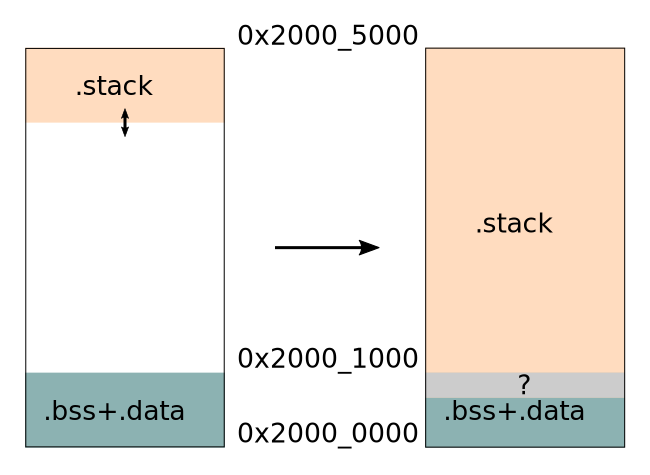
\includegraphics[width=0.9\textwidth]{obrazky/flip_overflow}
        \caption{Memory arrangement which causes memory corruption on stack overflow\cite{knurling_project_knurling-rsflip-link_2021}.}
        \label{fig:fliplink_orig}
    \end{minipage}\hfill
    \begin{minipage}[t]{0.45\textwidth}
        \centering
        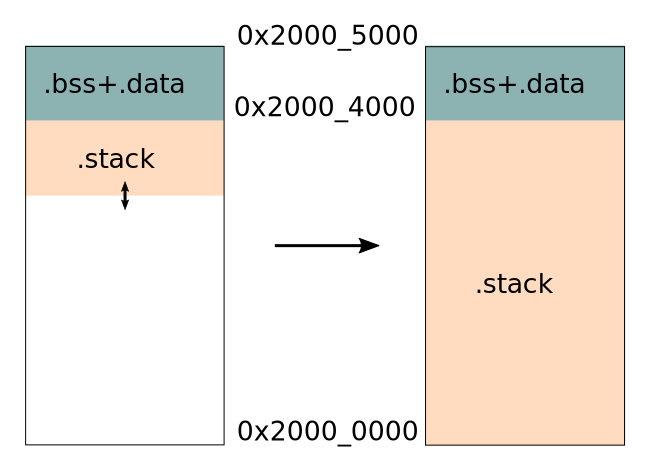
\includegraphics[width=0.9\textwidth]{obrazky/flip_flipped}
        \caption{Memory arrangement which causes hardware exception instead of corrupted memory\cite{knurling_project_knurling-rsflip-link_2021}.}
        \label{fig:fliplink_changed}
    \end{minipage}
\end{figure}

\subsection{Testing and CI}
\label{subsec:testing_ci}
While we already talked about testing in the Sections~\ref{subsec:testing} and \ref{subsubsec:defmttest}, we believe that there is more information about testing embedded Rust software and \acs{ci} (\acl{ci}).

There are two different types of tests that can be run for embedded software - tests, that can be run without the hardware, and tests that must be run on the target hardware as the code is dependent on it.
The tests that are independent on the target hardware can be tested using the standard Rust testing harness via for example \textbf{cargo test}, on the other hand to run these tests, a target that supports \textbf{std} is required, which might require some project structure changes.
As for the tests that must run on the target hardware, the \textbf{defmt-test} test harness can be utilized.
Approaches for testing these parts of the embedded firmware can be found here\cite{aparicio_testing_nodate,aparicio_testing_nodate-1}.
Hardware in the loop-testing is also possible\cite{schievink_running_nodate}.

Nowadays, it is also possible to run the tests as part of the project \acs{ci} workflow.
Apart from running tests, it is also possible to build the firmware as the only thing required is the Rust compiler with proper toolchain installed\cite{vahter_release_nodate}.
It is also possible to release the firmware, generate documentation and perform additional code checks on the codebase\cite{chiovoloni_few_2020}.

\section{Embedded Rust Advantages and Disadvantages}
\label{sec:embedded_rust_reasoning}
Many of the reasons why we believe that Embedded Rust is the right choice for embedded development have already been described in the previous sections, but let us sum up what we believe are the most important points.
\begin{itemize}
    \item The Rust language itself promotes and ensures code that is not prone to memory safety problems and data races.
    \item The Rust language ecosystem is large and integration of libraries is seamless and promotes code reuse.
    \item There are advanced and modern features in the language, making it easier to write safer and more expressive code.
    \item A lot of the abstractions provided by the programming language are zero-cost, meaning that they consume no additional resources.
    \item The embedded Rust ecosystem is vast and contains well-thought-out solutions to difficult problems in embedded - see Section~\ref{subsec:mut_shared_state} on \acs{rtic}.
    \item The embedded Rust teams seek to utilize the modern programming features, such as async/await and generics - see Section~\ref{subsec:async} on async/await.
    \item Some of the harder parts embedded are already developed and ready to use - such as USB and Ethernet drivers, with the community aiming to solve these hard problems having a language that helps mitigate common programming mistakes.
    \item The embedded tooling is gradually improving and in some ways it has already surpassed tooling in classical embedded languages - see the Section~\ref{subsec:tooling} on the tooling.
    \item Testing embedded systems with the Rust language is developed and testing the firmware is easy, even in the \acs{ci}.
\end{itemize}

On the other hand, there are some disadvantages of using embedded Rust:
\begin{itemize}
    \item The resulting binaries can be quite large (10s of kB), making it harder to run on lower end \acs{mcu}s.
    \item The support for debugging using GDB exists, but is not very ergonomic.
    \item The support for embedded in commonly used \acs{ide}s is low and sometimes for example autocomplete of registers can fail.
\end{itemize}
